\section{Verwendet Hardware}
\label{sec:verwendeteHardware}
Als Zielplattform für diese Thesis dient ein Raspberry Pi 4B. Dieser wird unter anderem deswegen
verwendet, da es im Labor Embedded Systems 2 der Hochschule Offenburg verwendet wird, aber auch,
da es sehr gut im Open Embedded Systems bereich eingesetzt werden kann. Der Raspberry Pi 4B
verfügt dabei, unter anderem, über die folgenden technischen Spezifikationen: \cite{RasberryPiSpecs}
\begin{itemize}
    \item 1,5 GHz ARM Cortex-A72 Quad-Core-CPU
    \item 1 GB, 2 GB oder 4 GB LPDDR4 SDRAM
    \item Gigabit LAN RJ45 (bis zu 1000 Mbit)
    \item Bluetooth 5.0
    \item 2x USB 2.0 / 2x USB 3.0
    \item 2x microHDMI (1x 4k @60fps oder 2x 4k @30fps)
    \item 5V/3A @ USB Typ-C
    \item 40 GPIO Pins
    \item Mikro SD-Karten slot
\end{itemize}
Und wird mit dem \emph{Raspbian Buster with desktop} auf der SD-Karte betrieben.
\newline
Um noch mehr Funktionalität aufbringen zu können, wurde auf dem Raspberry Pi ein
\emph{RPI SENSE HAT Shield} aufgesteckt. Mit hilfe des \emph{RPI SENSE HAT Shield} können dann
unter anderem Daten wie zum Beispiel die momentane Temperatur oder auch die momentane
Luftfeuchtigkeit gewonnen werden. Zudem ist auf dem SENSE HAT noch eine 8x8 LED-Matrix enthalten
und ein Joystick mit 5 knöpfen, die angesteuert werden können.
\begin{figure}[h]
    \centering
    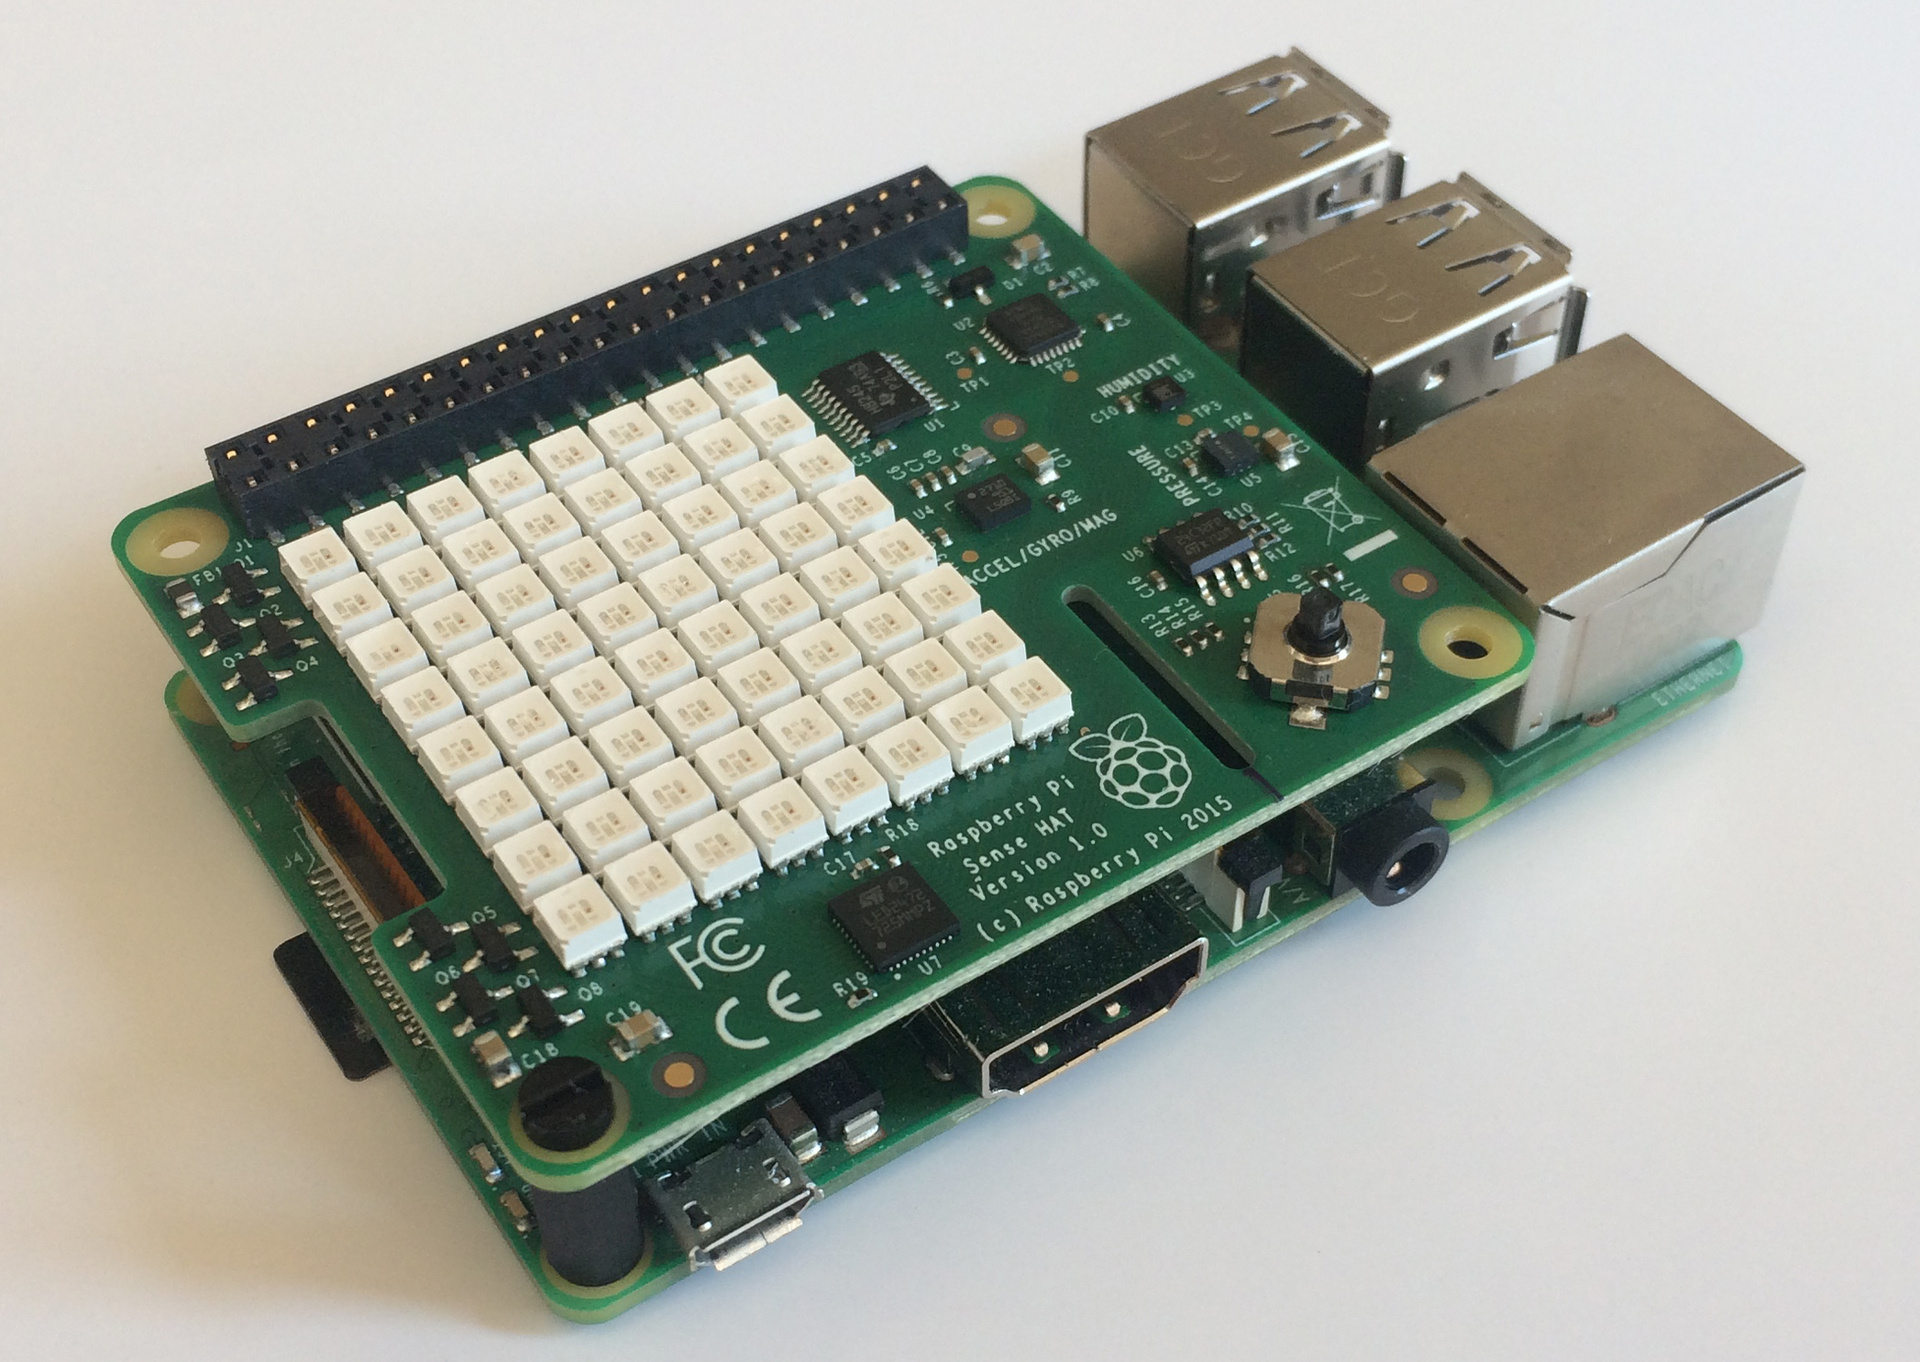
\includegraphics[width=0.5\textwidth, center]{Einleitung/pi-sense}
    \caption[Raspberry Pi 4 B]{Verwendeter Raspberry Pi}
    \label{img:piSense}
\end{figure}

